\documentclass{article}
\usepackage{amsmath}
\usepackage[utf8]{inputenc}
\usepackage{graphicx}
\usepackage{verbatim}
\usepackage{float}
\usepackage[makeroom]{cancel}
\usepackage[english]{babel}
\usepackage{textcomp}
\usepackage{gensymb}
\usepackage{color}
\usepackage{subcaption}
\usepackage{caption}
\usepackage{hyperref}
\usepackage{physics}
\usepackage{dsfont}
%\usepackage{amsfonts}
\usepackage{listings}
\usepackage{multicol}
\usepackage{units}

% From Eirik's .tex
\usepackage{epstopdf}
\usepackage{cite}
\usepackage{braket}
\usepackage{url}
\bibliographystyle{plain}

\usepackage{algorithmicx}
\usepackage{algorithm}% http://ctan.org/pkg/algorithms
\usepackage{algpseudocode}% http://ctan.org/pkg/algorithmicx

\usepackage[margin=1cm]{caption}
\usepackage[outer=1.2in,inner=1.2in]{geometry}
% For writing full-size pages
%\usepackage{geometry}
%\geometry{
%  left=5mm,
%  right=5mm,
%  top=5mm,
%  bottom=5mm,
%  heightrounded,
%}

% Finding overfull \hbox
\overfullrule=2cm

\lstset{language=IDL}
 %\lstset{alsolanguage=c++}
\lstset{basicstyle=\ttfamily\small}
 %\lstset{backgroundcolor=\color{white}}
\lstset{frame=single}
\lstset{stringstyle=\ttfamily}
\lstset{keywordstyle=\color{red}\bfseries}
\lstset{commentstyle=\itshape\color{blue}}
\lstset{showspaces=false}
\lstset{showstringspaces=false}
\lstset{showtabs=false}
\lstset{breaklines}
\lstset{aboveskip=20pt,belowskip=20pt}

\lstset{basicstyle=\footnotesize, basewidth=0.5em}
\lstdefinestyle{cl}{frame=none,basicstyle=\ttfamily\small}
\lstdefinestyle{pr}{frame=single,basicstyle=\ttfamily\small}
\lstdefinestyle{prt}{frame=none,basicstyle=\ttfamily\small}
% \lstinputlisting[language=Python]{filename}


\definecolor{codepurple}{rgb}{0.58,0,0.82}
\definecolor{backcolour}{rgb}{0.95,0.95,0.92}
\definecolor{dkgreen}{rgb}{0,0.6,0}
\definecolor{gray}{rgb}{0.5,0.5,0.5}
\definecolor{magenta}{rgb}{0.58,0,0.82}

\lstdefinestyle{pystyle}{
  language=Python,
  aboveskip=3mm,
  belowskip=3mm,
  columns=flexible,
  basicstyle={\small\ttfamily},
  backgroundcolor=\color{backcolour},
  commentstyle=\color{dkgreen},
  keywordstyle=\color{magenta},
  numberstyle=\tiny\color{gray},
  stringstyle=\color{codepurple},
  basicstyle=\footnotesize,
  breakatwhitespace=false,
  breaklines=true,
  captionpos=b,
  keepspaces=true,
  numbers=left,
  numbersep=5pt,
  showspaces=false,
  showstringspaces=false,
  showtabs=false,
  tabsize=2
}

%%%%%%%%%%%%%%%%%%%%%%%%%%%%%%%%
% Self made macros here yaaaaaay
\newcommand\answer[1]{\underline{\underline{#1}}}
\newcommand\pd[2]{\frac{\partial #1}{\partial #2}}
\newcommand\red[1]{\textcolor{red}{\textbf{#1}}}
\newcommand\numberthis{\addtocounter{equation}{1}\tag{\theequation}}
% Usage: \numberthis \label{name}
% Referencing: \eqref{name}

% Some matrices
\newcommand\smat[1]{\big(\begin{smallmatrix}#1\end{smallmatrix}\big)}
\newcommand\ppmat[1]{\begin{pmatrix}#1\end{pmatrix}}

%%%%%%%%%%%%%%%%%%%%%%%%%%%%%%%%%
% Eirik's self made macros
\newcommand{\s}{^{*}}
\newcommand{\V}[1]{\mathbf{#1}}
\newcommand{\husk}[1]{\color{red} #1 \color{black}}
\newcommand{\E}[1]{\cdot 10^{#1}}
\newcommand{\e}[1]{\ \text{#1}}
\newcommand{\tom}[1]{\big( #1 \big)}
\newcommand{\Tom}[1]{\Big( #1 \Big)}
\newcommand{\tomH}[1]{\big[ #1 \big] }
\newcommand{\TomH}[1]{\Big[ #1 \Big]}
\newcommand{\tomK}[1]{ \{ #1 \} }
\newcommand{\TomK}[1]{\Big\lbrace #1 \Big\rbrace}
\newcommand{\bigabs}[1]{\left| #1 \right|}

% Section labeling
\usepackage{titlesec}% http://ctan.org/pkg/titlesec
\renewcommand{\thesubsection}{\arabic{subsection}}

% Title/name/date
\title{FYS4150 - Project 5\\$N$-body simulation of an open galactic cluster}
\author{Simen Nyhus Bastnes \& Eirik Ramsli Hauge}
\date{9. December 2016}

\begin{document}
\maketitle
\begin{abstract}
\begin{figure}[H]
\centering

\includegraphics[scale=0.5]{totoro.jpg}
\end{figure}
\end{abstract}
\subsection{Introduction}
In this project we will attempt to develop code that can be used for gravitational $N$-body simulations. Taking inspiration from an article by M. Joyce and co-workers \red{cite}, we will build a simple model of an open galactic cluster.
\\\\
An open cluster is a group consisting of up to a few thousand gravitationally bound stars, created from the collapse of a molecular cloud, and are usually found in the arms of spiral galaxies or in in irregular galaxies. The collapse of the cloud leads to a burst of star formation. As the stars of the cluster are of similar age and chemical composition, they are very import objects in the study of stellar evolution. Once formed, they gradually dissipate as members are ejected due to random interactions with other clusters, clouds of gas, or internal collisions.
\\\\
First, we look at some of the physics behind our model, making sure to find ideal units to fit our timescale. Running our model for $N = 100$ particles, we check the stability of our system, and find an ideal smoothing function for the gravitational force to remove some of the numerical instabilities. Having done that, we check how long the system takes to stabilize, conservation of energy, and checking the fraction of particles ejected from the system. Looking at only the bound particles, we can check if our results are consistent with the virial theorem.
\red{write motivation for why N body simulations}
\\\\
Finally, we increase the number of particles while keeping the total mass constant, to see how the radial density looks like. This can then be compared to well known profiles such as the Navarro-Frenk-White profile.

\subsection{Theory}

\subsubsection{N-body simulation}
In order to make our model of an open cluster, we will first look at some of the assumptions we make.
\begin{itemize}
  \item Consists of $N$ separate particles only interacting with each other via the Newtonian gravitational force. The force between two particles are then
    \begin{align*}
      F_G = -\frac{G M_1, M_2}{r^2}\numberthis\label{eq:newton}
    \end{align*}
    where $G$ is the gravitational constant, $r$ is the distance between the particles, and $M_1$, $M_2$ is the mass of the particles. For most of the project, we will be looking at $N=100$ particles.
  \item Since the only interaction is the gravitational force, the system is collisionless. If the probability of interactions between particles is low, then collisions have no significant effect on the results. For very large $N$, this might not hold as well.
  \item The particles start with little or no initial velocity, so-called \textit{cold collapse}.
  \item The particles are uniformly distributed within a sphere of radius $R_0 = 20$ ly. Masses are randomly distributed by a Gaussian distribution around $10\,M_{\odot}$ with a deviation of one solar mass.
\end{itemize}
Earlier this fall, we made a model of our solar system. \red{cite report 3} We recall that for a system only affected by Newtonian gravity, Newton's second law of motion gives us the following differential equations for particle $i$
\begin{align*}
  \frac{d^2\mathbf{r_i}}{dt^2} &= \sum\limits_{j\neq i}\frac{F_G(\mathbf{r}_{ij}, M_i,M_j)}{M_i}\numberthis\label{eq:diff_eq}
\end{align*}
where $\mathbf{r}$ is a three-dimensional vector in $(x,y,z)$, and we sum over the gravitational contribution of the other particles. We note that the length and timescale should be adjusted to units more fit for the dynamics of the system.\\\\
For the length scale, we can use lightyears, as the particles are initially uniformly distributed inside a sphere of radius $R_0 = 20$ ly. In order to find units of time that fit the timescale however, we will take a short detour into non-linear perturbation theory and cosmology.
% def metal():

\subsubsection{The spherical top-hat model}
While solving non-linear perturbation theory analytically can be difficult (or impossible), there does exists an analytical solution for the so-called ``\textit{spherical top-hat}'' model \red{cite cosmo notes}. In this model, we look at a spherical perturbation of radius $R$, with a uniform density inside. It can be shown that this model has a parametrised solution
\begin{align*}
  R &= A(1-\cos\theta)\numberthis\label{eq:top-hat}\\
  t &= B(\theta-\sin\theta)\\
  &A^3 = GMB^2 
\end{align*}
From equation \eqref{eq:top-hat}, we see that the sphere reaches a maximum at $\theta = \pi$, at time $t=\pi B$ (also referred to as turn-around). The sphere collapses completely at $\theta = 2\pi$, at time $t = 2\pi B$. At $\theta = \tfrac{3\pi}{2}$, the model virializes at radius $1/2 R_0$. For the peak radius
\begin{align*}
  R(\theta = \pi) &= 2A = R_0\\
  t(\theta = \pi) &= \pi B
\end{align*}
Solving for $B$
\begin{align*}
  B &= \frac{A^{3/2}}{\sqrt{GM}}
  \intertext{Using that the density of the perturbation is given by $\rho_0 = M/V = M/(4/3\pi R_0^3)$}
  B &= \frac{(R_0/2)^{3/2}}{\sqrt{G\frac{4\pi R_0^3\rho_0}{3}}}\\
  B &= \sqrt{\frac{3}{32\pi G\rho_0}}
\end{align*}
Since our simulation starts with cold collapse (at turn-around $\theta = \pi$), the time it takes to collapse is
\begin{align*}
  t_{\text{coll}} &= t_{2\pi} - t_{\pi}\\
  t_{\text{coll}} &= 2\pi B - \pi B = \pi B
  \intertext{inserting the expression we found for $B$, we get the collapse time}
  t_{\text{coll}} &= \sqrt{\frac{3\pi}{32G\rho_0}}\numberthis\label{eq:t_coll}
\end{align*}
As this time, $t_{\text{coll}}$ is an analytical expression for collapse in the \textit{spherical top-hat model}, this is a much more fitting timescale to probe our system with compared to seconds or years.\\\\
In order to make use of this, we need to scale equation \eqref{eq:newton} in these units, specifically $G$. Rewriting equation \eqref{eq:t_coll} gives us
\begin{align*}
  G &= \frac{3\pi}{32\rho_0t_{\text{coll}}^2}
  \intertext{Scaling so that we are looking at timescales of order $t_{\text{coll}}$, and inserting $\rho_0 = 4/3\pi R_0^3$}
  G &= \frac{\pi^2R_0^3}{8M_{tot}} = \frac{\pi^2R_0^3}{8N\mu} \numberthis\label{eq:G}
\end{align*}
where $N$ is the number of particles, and $\mu$ is the average mass (in solar masses) per particle.\\\\
Inserting equation \eqref{eq:G} into the differential equation given by \eqref{eq:diff_eq} gives us the units $[\text{ly}/t_{\text{coll}}]$, which is what we wanted.
%Page 18ish in cosmo1.5 lecture notes\\
%collapse time, spherical top hat model, virialization.
%Sphere completely collapses at $\theta = 2\pi$ \red{add image maybe?}

\subsubsection{Numerical instabilities}
Since we will be solving the system numerically, we have to be aware of some of the problems of doing so. In this project, we will focus on the numerical instability that arises when two particles come very close to each other. When two particles get close to each other, the accelerations get large, and unless we have very small timesteps, the trajectory of a particle is not calculated accurately. To deal with this, we will introduce a very simple smoothing function by modifying the Newtonian force \eqref{eq:newton}
\begin{align*}
  F_{\text{mod}} &= \frac{GM_1M_2}{r^2 + \varepsilon^2} \numberthis\label{eq:newton_mod}
\end{align*}
where $\varepsilon$ is a small real constant that causes equation \eqref{eq:newton_mod} to be finite on short length scales. While adding this smoothing factor smooths out the instabilities, it also means that on length scales smaller than $\varepsilon$, the trajectories are not integrated accurately. This means that we should make sure to set the smoothing factor $\varepsilon$ to a length so that 1) instabilities are smoothed out, and 2) the inaccuracy in the trajectory does not play a significant part of the macroscopic evolution of the system.\\\\
As we discussed earlier, we assume the system to be collisionless, and that collisions (or close encounters) should not affect the system much. Since our particles does not represent point particles, but mass distributions with some finite radius, a really close encounter between two particles might not be fully collisionless. The smoothing factor does then in a sense represent the fact that our system is not fully collisionless, but the magnitude of it is most likely considerably larger than the scale at which collisions become relevant.\\\\
Finding an ideal size for $\varepsilon$ can be difficult. A simple way to evaluate this is to first find the mean interparticle distance. \red{cite Joyce full}
\begin{align*}
  l &\equiv \bigg(\frac{3V}{4\pi N}\bigg)^{1/3} = \frac{R_0}{N^{1/3}} \numberthis\label{eq:mean_dist}
\end{align*}
where $R_0$ is the initial radius of the sphere, and $N$ is the number of particles. Since this is the average distance between the particles at the start of the simulation, we should make sure that our choice of $\varepsilon$ is significantly less than $l$, as it limits how small the structure is allowed to collapse. For example, for the situation $R_0 = 20$ and $N = 100$, we have $l \approx 4.3$.

%try to find fitting size order from mean particle distance and refer to article
\subsubsection{Particle ejection}
Due to looking at a \textit{cold collapse}, all particles start with a negative energy, but as the system evolves, some of the particles can end up with a positive energy, and completely escape from the system. We can therefore identify these ejected particles by comparing the per particle kinetic and potential energy, and identifying which particles have a total energy greater than zero
\begin{align*}
  E_{i,\text{tot}} = K_i + V_i > 0 \numberthis\label{eq:ejection}
\end{align*}
where $K_i$ and $V_i$ is the kinetic and potential energy for particle $i$.\\\\
The energy taken away from the system by particle ejection can be found by energy conservation and that once the system stabilizes, the potential energy of the ejected particles and the interaction between bound and ejected particles is negligible
\begin{align*}
  E_0 &= V_b + K_b + K_f \numberthis\label{eq:energy_ejection}
\end{align*}
where $E_0$ is the initial energy of the system, $V_b$ and $K_b$ is the kinetic and potential energy of the particles that are gravitationally bound, and $K_f$ is the kinetic energy of the ejected particles.
$K_f$ can be found as discussed earlier in equation \eqref{eq:ejection}.

\subsubsection{Virial theorem}
For a bound gravitational system in equilibrium, the virial theorem says that
\begin{align*}
  2\langle K\rangle &= -\langle V\rangle \numberthis\label{eq:virial}
\end{align*}
where $\langle K\rangle$ is the time-average kinetic energy of the system, and $\langle V\rangle$ is the time-average potential energy. By the ergodic hypothesis, we can assume that an average over a large enough system should give the same result as the time average. Thus we have
\begin{align*}
  2K_b &= -V_b \numberthis\label{eq:virial2}
\end{align*}
where $K_b$ and $V_b$ are the energies for the bound particles, and can be found from equation \eqref{eq:energy_ejection}

\subsubsection{Radial density of particles}
For an approximately spherical symmetric collapsed halo (virialized structure), the radial density profile can often be fit very well with the simple expression
\begin{align*}
  n(r) = \frac{n_0}{\Big(1+(\frac{r}{r_0})^4\Big)} \numberthis\label{eq:radial_dist}
\end{align*}
where $n_0$ and the scale radius $r_0$ has some dependency on the number of particles $N$.\\\\
The well-known Navarro-Frenk-White profile can also be used to compare with results.
\begin{align*}
  \rho(r) &= \frac{\rho_0}{\frac{r}{r_0}\Big(1+\frac{r}{r_0}\Big)^2}\numberthis\label{eq:NFW}
\end{align*}
where $\rho_0$ and $r_0$ depends on $N$ in some way.
\subsubsection{Numerical solving}
In order to solve the system numerically, we will employ the Velocity Verlet method. A full derivation of the Velocity Verlet method can be found in \red{cite project 3}, where the following algorithm is also found.
\begin{algorithm}[H]
\small
\caption{Velocity Verlet}\label{alg:VelVerlet}
\begin{algorithmic}[1]
\For{$i = 0, n$}
\State $r_{i+1} = r_i + v_i h + \frac{1}{2} a_i h^2$
\State $a_{i+1} = F_{G, r_{i+1}}/m$
\State $v_{i+1} = v_i + \frac{1}{2} h (a_i + a_{i+1})$
\EndFor
\end{algorithmic}
\end{algorithm}
\subsection{Experimental}
The programs used in this project can be found in the GitHub repository \cite{GitHub}, in the \texttt{/src/} folder. When running the program it takes 4 command line arguments: \texttt{N}, \texttt{t\_coll}, \texttt{dt} and \texttt{eps}. \texttt{N} is the number of stars in our cluster, \texttt{t\_coll} is our time unit, based on the collision time, \texttt{dt} is the time step and \texttt{eps} is the smoothing factor used in the force calculation. All data written to file by the main program are stored in \texttt{/benchmarks/} where most of the data analysis were done by python programs stored in \texttt{/python/} and the figures and gifs can be found in \texttt{/figures/}. \\ \\
The simulation starts by randomly positioning different stars inside a sphere with radius R = 20 light years. Each star will have an individual mass where the total mass is forced to be 1000 solar masses and an initial velocity set to be 0 in all directions. \\
Once all the positions and masses have been set, we can find the forces acting between them. While using velocity verlet to simulate the behaviour we can also find the individual kinetic and potential energy of each star as well as the total kinetic and potential energy of the system. 
\subsection{Results}
%%%%%%%%%%%%%%%%%%%%%%%%%%%%%
%%%         task b        %%%
%%%%%%%%%%%%%%%%%%%%%%%%%%%%%
A simulation for N = 100 particles over a time of 5 collision times with a time step of 0.001 and no smoothing factor is plotted in figure \ref{fig:noepsmuchtime} for different times during the simulation. From these figures and the figure \ref{fig:noeps} we can see that without a smoothing factor we will never reach an equilibrium.
\begin{figure}[H]
\centering
\begin{subfigure}{0.49\textwidth}
	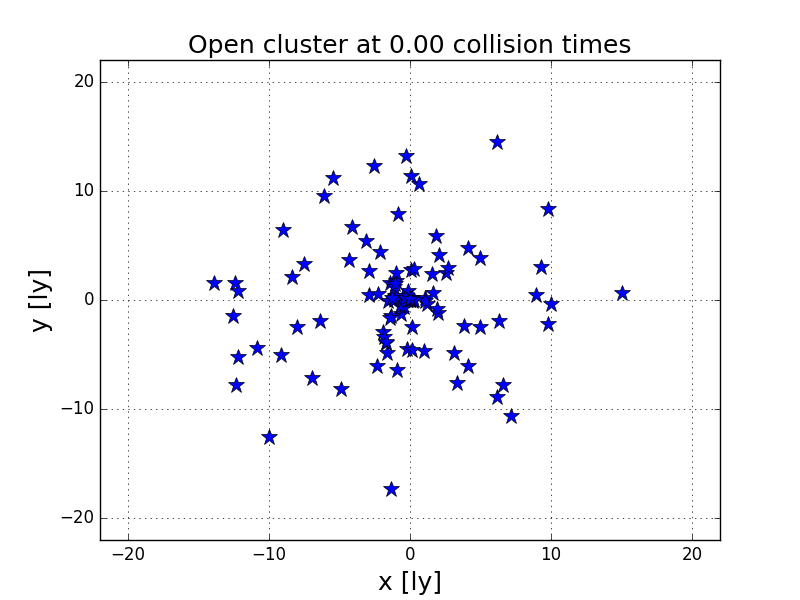
\includegraphics[scale=0.33]{{../figures/taskb/N100/plot_N100_time0.00}.png}
	\caption{At time 0.00 collision times}
	\label{subfig:noepsmuchtime1}
\end{subfigure}
\begin{subfigure}{0.49\textwidth}
	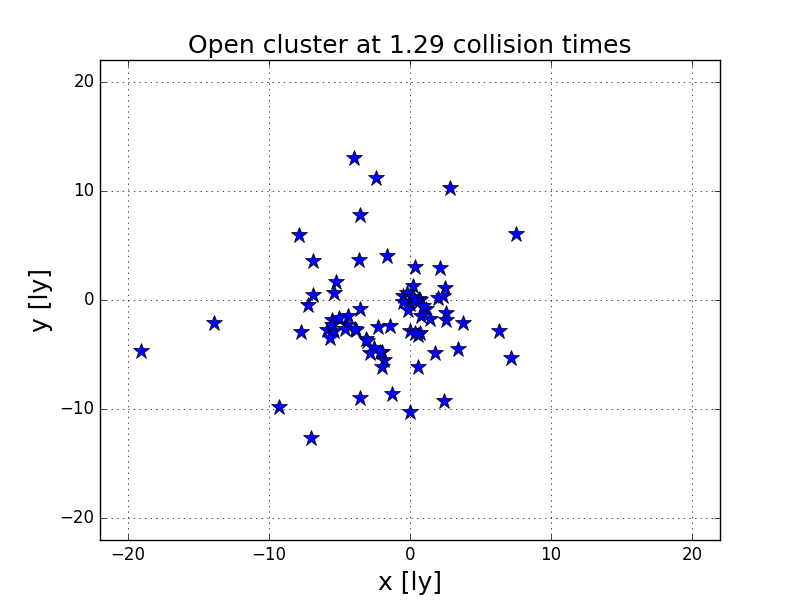
\includegraphics[scale=0.33]{{../figures/taskb/N100/plot_N100_time26.00}.png}
	\caption{At time 1.29 collision times}
	\label{subfig:noepsmuchtime2}
\end{subfigure}
\qquad
\begin{subfigure}{0.49\textwidth}
	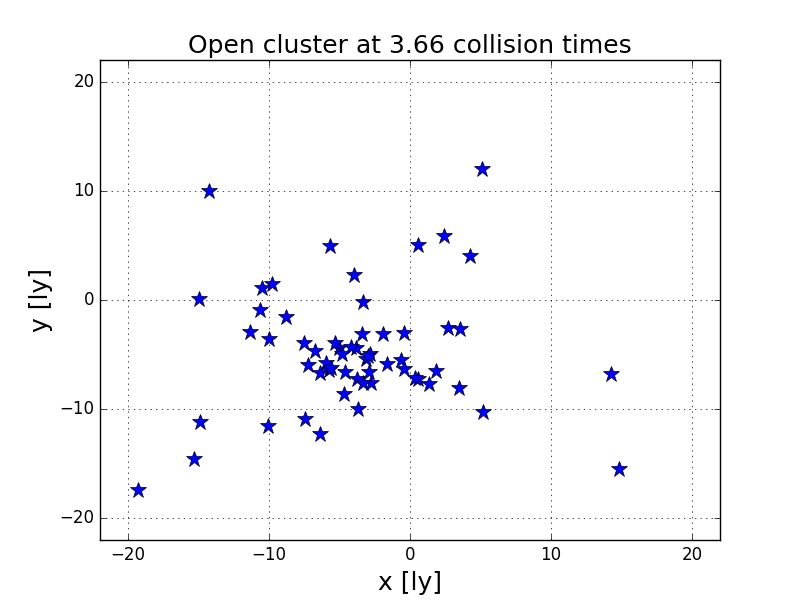
\includegraphics[scale=0.33]{{../figures/taskb/N100/plot_N100_time74.00}.png}
	\caption{At time 3.66 collision times}
	\label{subfig:noepsmuchtime3}
\end{subfigure}
\begin{subfigure}{0.49\textwidth}
	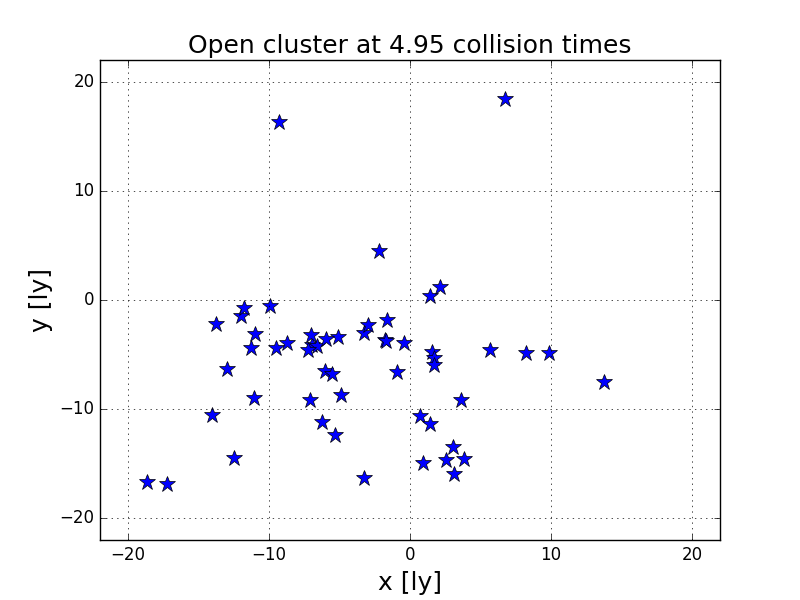
\includegraphics[scale=0.33]{{../figures/taskb/N100/plot_N100_time100.00}.png}
	\caption{At time 4.95 collision times}
	\label{subfig:noepsmuchtime4}
\end{subfigure}
\caption{Position of each star in 2D as a function of time.}
\label{fig:noepsmuchtime}
\end{figure}
%%%%%%%%%%%%%%%%%%%%%%%%%%%%%
%%%         task c        %%%
%%%%%%%%%%%%%%%%%%%%%%%%%%%%%
Letting our program run for different number of particles we found the total energy, the fraction of particles with positive total energy and the kinetic energy of the escaped particles. These results are shown below in figure \ref{fig:noeps}.

\begin{figure}[H]
\centering
\begin{subfigure}{0.49\textwidth}
	\includegraphics[scale=0.33]{{../figures/taskc/totenergy_N100}.png}
	\caption{Number of particles: 100}
	\label{subfig:noeps100}
\end{subfigure}
\begin{subfigure}{0.49\textwidth}
	\includegraphics[scale=0.33]{{../figures/taskc/totenergy_N200}.png}
	\caption{Number of particles: 200}
	\label{subfig:noeps200}
\end{subfigure}
\qquad
\begin{subfigure}{0.49\textwidth}
	\includegraphics[scale=0.33]{{../figures/taskc/totenergy_N500}.png}
	\caption{Number of particles: 500}
	\label{subfig:noeps500}
\end{subfigure}
\begin{subfigure}{0.49\textwidth}
	\includegraphics[scale=0.33]{{../figures/taskc/totenergy_N1000}.png}
	\caption{Number of particles: 1000}
	\label{subfig:noeps1000}
\end{subfigure}
\caption{Total energy (top), fraction of escaped particels (middle) and the kinetic energy of the escaped partivles (bottom) for different number of particles without a smoothing factor.}
\label{fig:noeps}
\end{figure}
%%%%%%%%%%%%%%%%%%%%%%%%%%%%%
%%%         task d        %%%
%%%%%%%%%%%%%%%%%%%%%%%%%%%%%
To find the best smoothing factor discussed above in the theory we used the trial and error method. For 200 stars with a time step of 0.001 and a time from 0 to 5 collision times we found the total energy as presented in figure \ref{fig:totalEnergy}
\begin{figure}[H]
\centering
\begin{subfigure}{0.49\textwidth}
	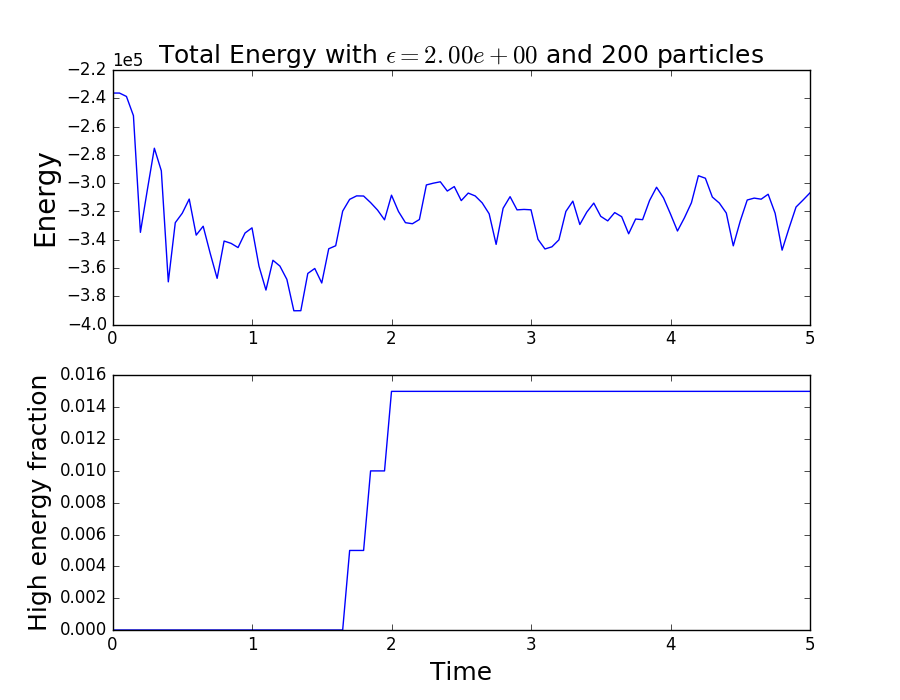
\includegraphics[scale=0.33]{{../figures/taskd/totenergy_eps2.00e+00_N200}.png}
	\caption{$\epsilon$ = 2.0}
	\label{subfig:eps2}
\end{subfigure}
\qquad
\begin{subfigure}{0.49\textwidth}
	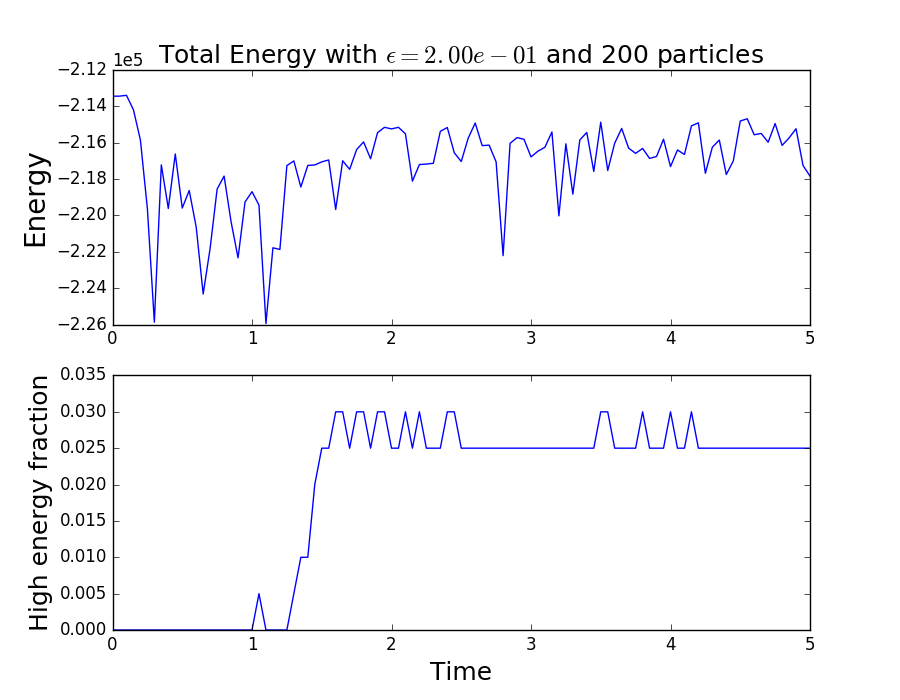
\includegraphics[scale=0.33]{{../figures/taskd/totenergy_eps2.00e-01_N200}.png}
	\caption{$\epsilon$ = 0.2}
	\label{subfig:eps0.2}
\end{subfigure}
\begin{subfigure}{0.49\textwidth}
	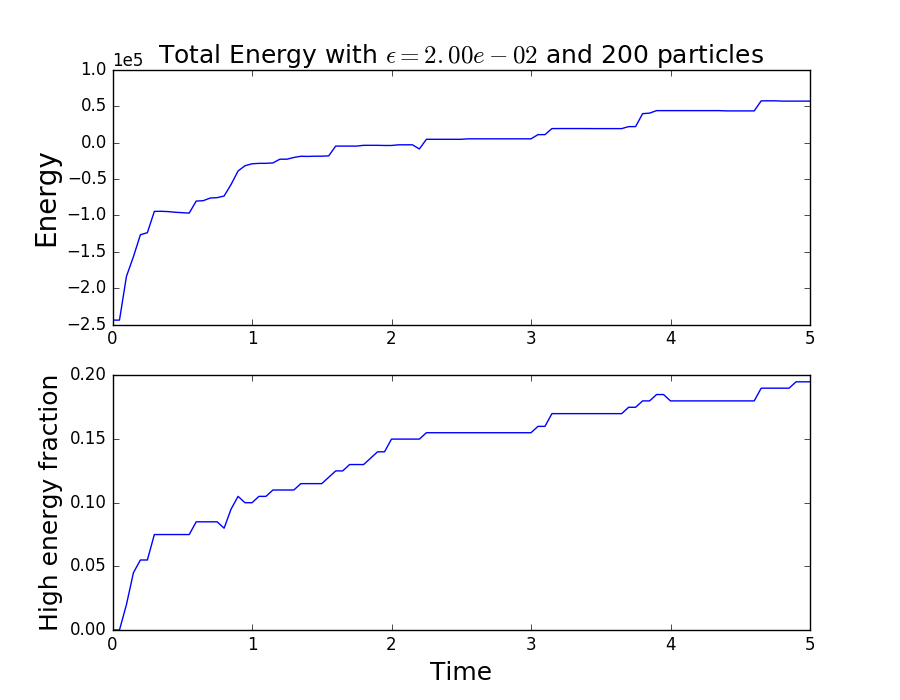
\includegraphics[scale=0.33]{{../figures/taskd/totenergy_eps2.00e-02_N200}.png}
	\caption{$\epsilon$ = 0.02}
	\label{subfig:eps0.02}
\end{subfigure}
\caption{Total energy (top) and fraction escaped particles (bottom) for different smoothing factors for a simulation of 200 particles.}
\label{fig:totalEnergy}
\end{figure}
As we now have found a better smoothing factor we can once again simulate for different number of particles and see the difference. By setting a smoothing factor of 0.1 and simulating for different number of particles with time step 0.001 and over a time period of 5 collisions times the graphs in figure \ref{fig:witheps}:
\begin{figure}[H]
\centering
\begin{subfigure}{0.49\textwidth}
	\includegraphics[scale=0.33]{{../figures/taskd/totenergy_N100}.png}
	\caption{Number of particles: 100}
	\label{subfig:witheps100}
\end{subfigure}
\begin{subfigure}{0.49\textwidth}
	\includegraphics[scale=0.33]{{../figures/taskd/totenergy_N200}.png}
	\caption{Number of particles: 200}
	\label{subfig:witheps200}
\end{subfigure}
\qquad
\begin{subfigure}{0.49\textwidth}
	\includegraphics[scale=0.33]{{../figures/taskd/totenergy_N500}.png}
	\caption{Number of particles: 500}
	\label{subfig:witheps500}
\end{subfigure}
\begin{subfigure}{0.49\textwidth}
	\includegraphics[scale=0.33]{{../figures/taskd/totenergy_N1000}.png}
	\caption{Number of particles: 1000}
	\label{subfig:witheps1000}
\end{subfigure}
\caption{Total energy (top), fraction of escaped particels (middle) and the kinetic energy of the escaped partivles (bottom) for different number of particles with a smoothing factor.}
\label{fig:witheps}
\end{figure}
%%%%%%%%%%%%%%%%%%%%%%%%%%%%%
%%%         task e        %%%
%%%%%%%%%%%%%%%%%%%%%%%%%%%%%
To see if we our results were consisten with the viral theorem, we checked if equation \eqref{eq:virial2} held for our system. The result are plotted in figure \ref{fig:viral}
\begin{figure}[H]
\centering
\begin{subfigure}{0.49\textwidth}
	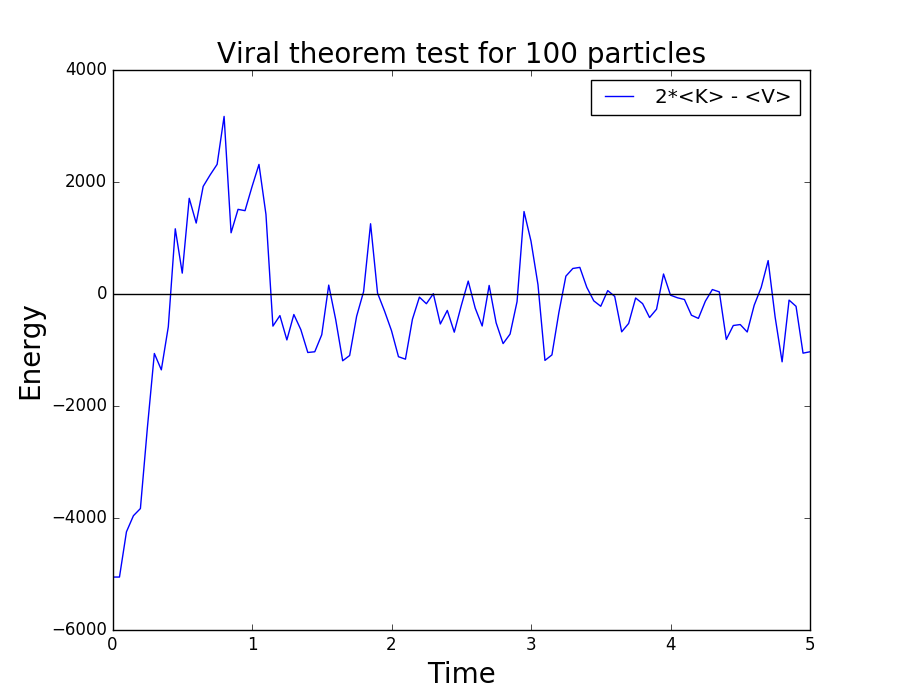
\includegraphics[scale=0.33]{{../figures/taske/viral_N100}.png}
	\caption{Number of particles: 100}
	\label{subfig:viral100}
\end{subfigure}
\qquad
\begin{subfigure}{0.49\textwidth}
	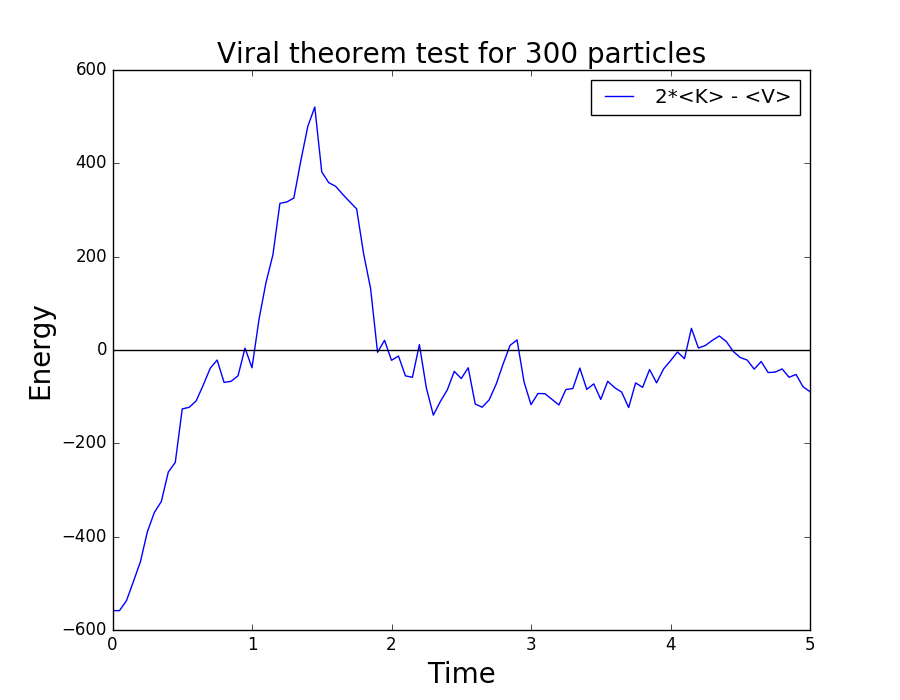
\includegraphics[scale=0.33]{{../figures/taske/viral_N300}.png}
	\caption{Number of particles: 300}
	\label{subfig:viral300}
\end{subfigure}
\begin{subfigure}{0.49\textwidth}
	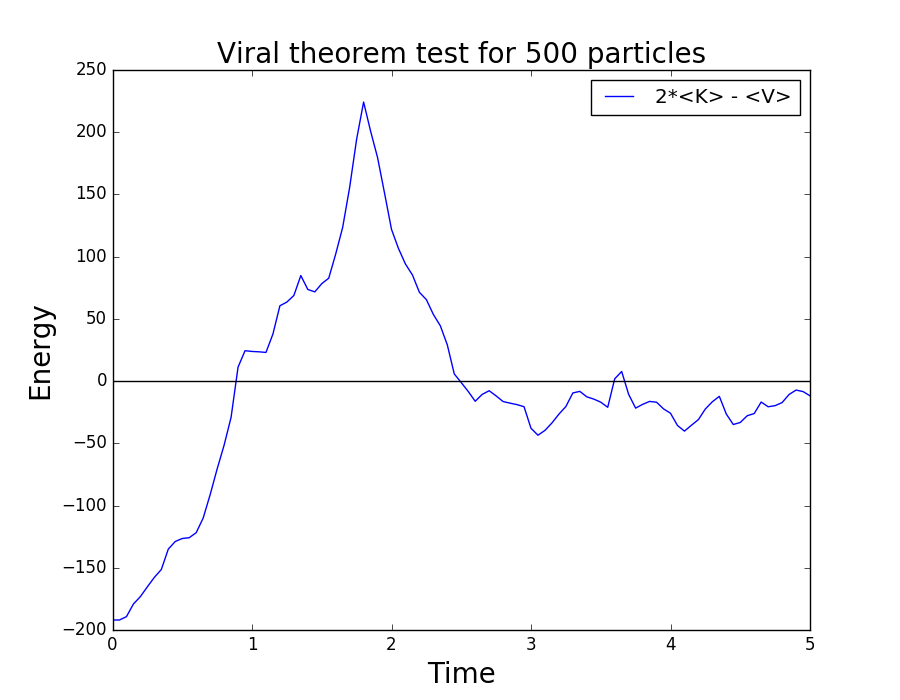
\includegraphics[scale=0.33]{{../figures/taske/viral_N500}.png}
	\caption{Number of particles: 500}
	\label{subfig:viral500}
\end{subfigure}
\caption{Test of the viral theorem. When the blue and black line crosses, we have fullfilled the viral theorem. The energies are the average of a large system.}
\label{fig:viral}
\end{figure}
%%%%%%%%%%%%%%%%%%%%%%%%%%%%%
%%%         task f        %%%
%%%%%%%%%%%%%%%%%%%%%%%%%%%%%
By simulating different number of particles with the same total mass we were able to find the radial density, mean distance from origo and the standard derivation of distance from origo (see figure \ref{fig:radialDens} and \ref{fig:meanstd})
\begin{figure}[H]
\centering
\begin{subfigure}{0.49\textwidth}
	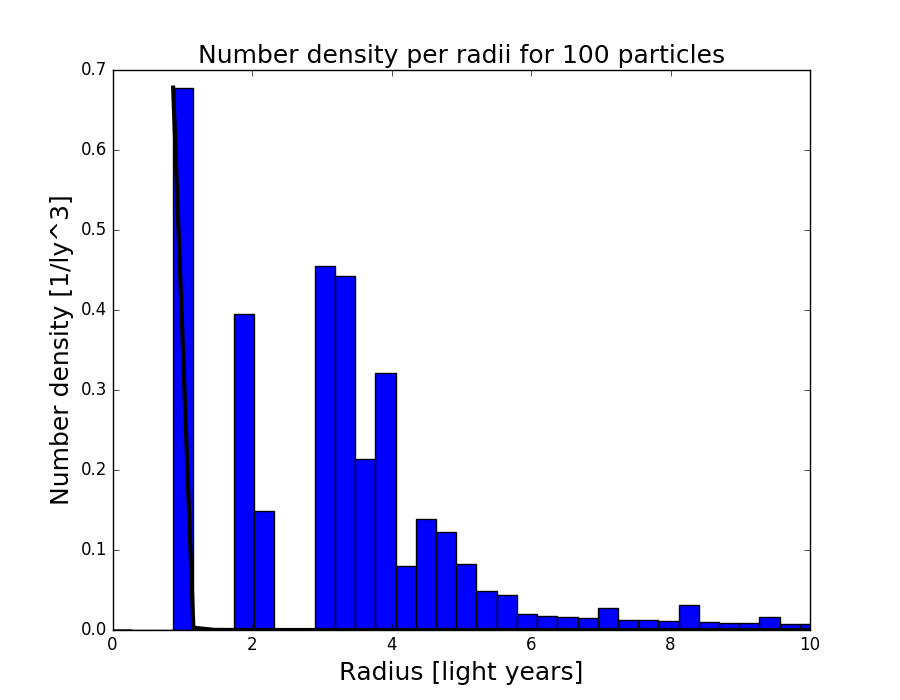
\includegraphics[scale=0.33]{{../figures/taskf/radialDens_N100}.png}
	\caption{Number of particles: 100}
	\label{subfig:radialDens100}
\end{subfigure}
\qquad
\begin{subfigure}{0.49\textwidth}
	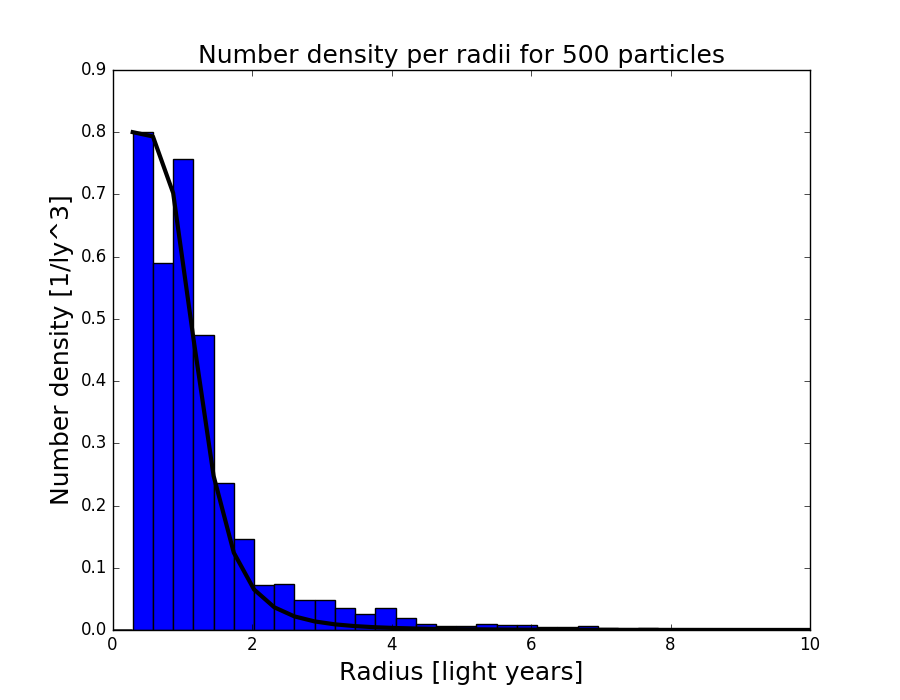
\includegraphics[scale=0.33]{{../figures/taskf/radialDens_N500}.png}
	\caption{Number of particles: 500}
	\label{subfig:radialDens500}
\end{subfigure}
\begin{subfigure}{0.49\textwidth}
	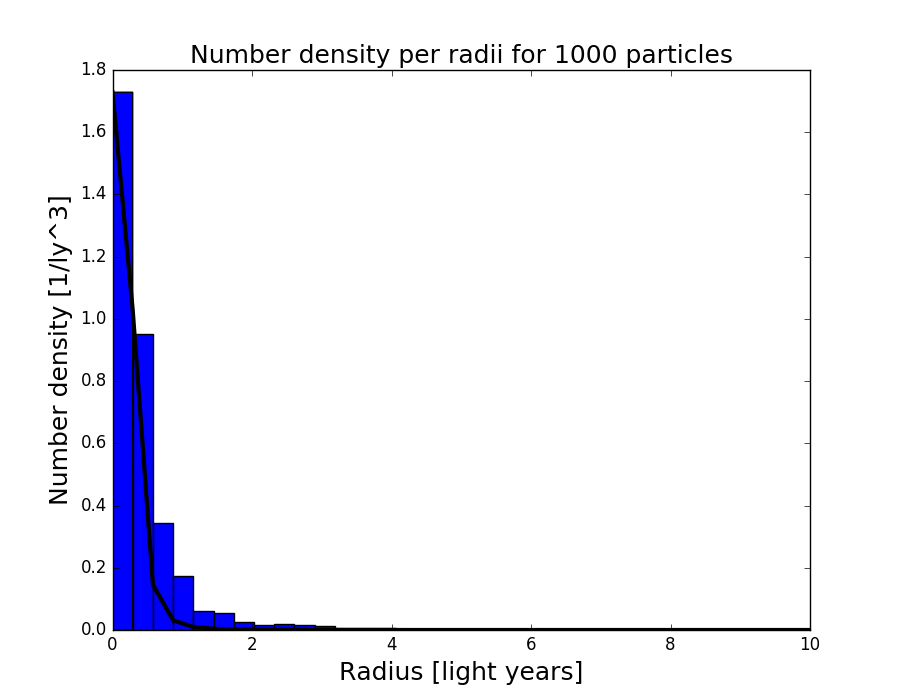
\includegraphics[scale=0.33]{{../figures/taskf/radialDens_N1000}.png}
	\caption{Number of particles: 1000}
	\label{subfig:radialDens1000}
\end{subfigure}
\caption{Radial density for different number of particles.}
\label{fig:radialDens}
\end{figure}
\begin{figure}[H]
\centering
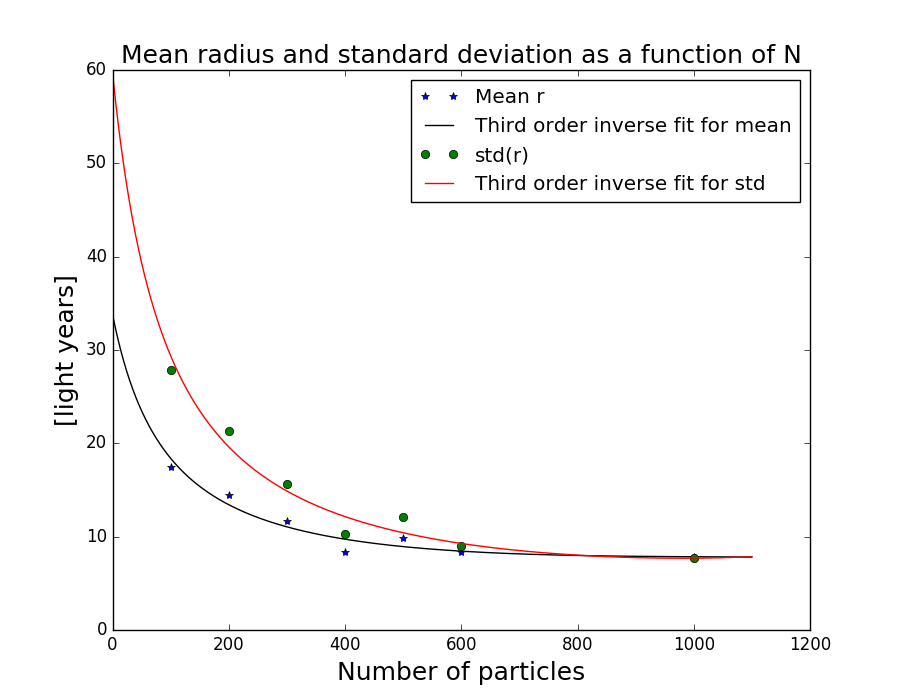
\includegraphics[scale=0.5]{{../figures/taskf/meanstd}.png}
\caption{Standard deviation and average distance from origo for all particles}
\label{fig:meanstd}
\end{figure}
\subsection{Discussion}
%%%%%%%%%%%%%%%%%%%%%%%%%%%%%
%%%         task a        %%%
%%%%%%%%%%%%%%%%%%%%%%%%%%%%%
The choice of time step was done by trial and error. From the extended report by Joyce \husk{cite Joyce full}, we found that they used a time step of 5.0e-05 during the collapse phase around $t_{coll}$, while 5.0e-4 during the other phases. We tried different values and found that a $dt$ of 1.0e-03 was a good time step, which both gave us a good resolution while also keeping the time usage of the program low.\\\\
In the limit $N \rightarrow \, \infty$ with a constant $\rho$ we get a continuous fluid. The system should then collapse into a singularity after one $t_{coll}$. However, we do not observe this collapse in our simulation. This is due to the fact that while we distribute our particles uniformly, it will not be fully isotropic for finite $N$, and the small deviations cause particles to miss the center, and shoot outwards again high velocity. The end result of this is that the system ``\textit{virializes}'' in an equilibrium state at a finite radius.% not all matter is on perfectly radial orbits. %With random distribution there will be many particles that do not go through the center, and even if they did there would be nothing there to stop it as it can not collide.
\\ \\
%%%%%%%%%%%%%%%%%%%%%%%%%%%%%
%%%         task b        %%%
%%%%%%%%%%%%%%%%%%%%%%%%%%%%%
%%%%%%%%%%%%%%%%%%%%%%%%%%%%%
%%%         task c        %%%
%%%%%%%%%%%%%%%%%%%%%%%%%%%%%
As we can see from figure \ref{fig:noeps} where $\varepsilon = 0$, the energy is never conserved nor is it stable and there is no point in discussing these plots in detail, as the numerical instabilities discussed earlier causes some particles to gain a lot of energy. Even with testing for time steps as small as 1.0e-6, the instabilities remain.
\\\\
The plots in figure \ref{fig:witheps}, where we have added a smoothing factor are much more interesting and we are especially interested in the middle and bottom ones for each simulation. Number of particles escaping and the kinetic energy of these particles are found using equation \eqref{eq:ejection} and we notice two trends. As the number of particles increases there seem to be a larger fraction of escaping particles. This is true up until 500 particles, but the fraction is a bit lower at 1000. The cause of this might either be that there are abnormalities in our measurements, this could easily be corrected by doing the simulation many times and the take an average, or it could be because the fraction increases for low values of $N$ and then it is more constant for larger values of $N$. By looking at the energy of the escaped particles we see a different story. Max values of each simulation at the equilibrium time (see below) seem to decrease as there are more particles added to the system. This means that with more particles, even though more are escaping, the ones that do escape have a lower kinetic energy per particle. As we keep the total mass of the system constant, each particle has less mass, and thus the difference could be attributed to this.
\\ \\
Once the system reaches equilibrium there are still some particles being ejected, as seen from the fraction of particles escaping, but this fraction becomes more and more stable for larger values of $N$.\\
The bottom part of the three plots for each $N$-values shows us the energy of the escaped particles. We notice that once equilibrium is reached the escaped kinetic energy slowly decreases over time. This is due to the fact that when the particle is defined as ejected ($E>0$), it is still affected gravitationally by the other particles. As time progresses, the ejected particles lose some kinetic energy as they work their way out of the gravitational potential.
\\ \\
The system seems in general to be more stable for larger values of $N$. If we were to do this experiment again we would likely use larger $N$-values, and do multiple simulations for each $N$-value. This time around however, we had exams in a lot of other courses and had only time for the simulations we have run.
\\ \\
%%%%%%%%%%%%%%%%%%%%%%%%%%%%%
%%%         task d        %%%
%%%%%%%%%%%%%%%%%%%%%%%%%%%%%
Due to the numerical instabilities that arises when two particles come very close, we implement a smoothing factor to our force calculations as shown in \eqref{eq:newton_mod}. The ideal value for the smoothing factor is a factor that is difficult to pinpoint. However, we would like it to be a couple of factors lower than the mean interparticle distance given by equation \eqref{eq:mean_dist}, but also large enough to smooth the instabilities enough. As we can see from the figures in \ref{fig:noeps} there were several values tried out for $N = 200$ which would have a mean interparticle distance of 3.42 light years. The value $\epsilon = $ 0.02 was clearly the worst. With no stabilization in the escaped particles and a total energy showing a increase rather than being stable, the value could not be used. $\epsilon = 0.2$ and $\epsilon = 2.0$ both show a stabilizing effect. The oscillation of the fraction of high energy particles for $\epsilon = 0.2$ could be a result of particles on the border of escaping, going back and forth. If we did this project again I would like to do this for even more values of N, finding a better way to determine $\epsilon$ and find the reason for the oscillating. \\
With a known vaue of $\epsilon$ for 200 N we redid the results from earlier tasks. The challenge here was to estimate a value of $\epsilon$ for every $N$. As the mean interparticle distance decreases for higher $N$, it should become smaller with larger $N$ and that for 0.2 was good for 200, we set the value to 0.1 before simulating 100, 200, 500 and 1000 particles. Ideally every values of $N$ should have its own $\epsilon$, but since we only know that it should be less than the mean interparticle distance and 0.2 worked for 200, we thought that 0.1 would be a good estimation for all these $N$-values, even though a more thorough evaluation of $\varepsilon$ should have been done. If we were to do this project again, it would be wise to find individual $\epsilon$ by comparing different values as in figure \ref{fig:noeps}, but as our results are not used any further, our estimation seems to be a good one. \\
These figures shows us that with a smoothing factor we can reach an equilibrium which differs in time for the different values of N that are placed randomly within the same volume and with the same total mass. By looking at the fraction of particles with positive energy, there seems to be an equilibrium at around 1 $t_{coll}$ for 100 particles, 1.6 $t_{coll}$ for 200, 2.5 $t_{coll}$ for 500 and 3.5 $t_{coll}$ for 1000 particles. This increase in equilibrium time is a bit weird as one would expect the equilibrium time to be approximately $t_{coll}$ for all $N$. The fact that we observe such a large difference tells us that something seems to be wrong, but we have not been able to see what. Once again we realize that if we were to do this again, the increasing equilibrium time is definitely something that should be looked at closer.\\
The addition of the smoothing factor can be justified to some extent, as discussed in the theory, by the fact that we do not look at point particles but rathermass distributions of some finite extent, and that we do not simulate collisions between the particles. This shows that we will not get an accurate representation of the trajectories at small length scales, but for our purposes in this project the simple smoothing correction is a good estimation as long as the system remains mostly collisionless. \\ \\
%%%%%%%%%%%%%%%%%%%%%%%%%%%%%
%%%         task e        %%%
%%%%%%%%%%%%%%%%%%%%%%%%%%%%%
From figure \ref{fig:viral} the virial theorem fits better and better for higher values of $N$. This makes sense as a larger $N$ means that kinetic and potential energy is closer to the time averaged energies, as discussed earlier. The difference from zero is however to large to ignore, at least for $N = 100$. This means that the virial theorem is mostly consistent with our results, but not quite and especially not for a small number particles. It might be the way we extract the energy for bound particles, but as we discussed earlier, once the system reaches equilibrium the ejected particles should not affect the gravitational energy of the system.  It might be that we have a fault in our simulation, or that the smoothing factor is not ideal. Some variation around zero is to be expected, but if we were to do the experiment again, attempting to improve these results should be done. But as the other parts of our program makes sense and our virial theorem test improves for larger values of N, it is reasonable to argue that we have something that works fairly well, but it is not ideal for small $N$ or that our energy is either extracted wrong or manipulated wrong by our calculations.
%%%%%%%%%%%%%%%%%%%%%%%%%%%%%
%%%         task f        %%%
%%%%%%%%%%%%%%%%%%%%%%%%%%%%%
\\\\
As we can see from figure \ref{fig:radialDens} the cluster is densest near origo. This is as expected, as most of the particles should form a structure at some finite radius. The solid line shows our best fit of the number density by equation \eqref{eq:radial_dist}, shifted to start at the maximum value on the histogram as our simulation does not allow for many particles to occupy the small volume near $r=0$, or if the anisotropy of the initial conditions makes the center-of-mass move. We see that the profile does fit our results fairly well when $r_0 \propto N^{-1/3}$, while $n_0$ is set to the maximum value of the histogram due to the fact that it is normalized. Finding an $N$ dependence on $n_0$ could have been done.\\\\
The mass density plotted versus radius is not included, as they were close to indistinguishable from the number density (figure \ref{fig:radialDens}). This is not surprising, given the fact that we only have one type of particle, where the mass is given by a gaussian distribution. We attempted to fit the NFW profile \eqref{eq:NFW} to the mass density, without success due to time constraints.\\\\
Figure \ref{fig:meanstd} shows that the mean radius decreases with increasing $N$. This is consistent with the results from \red{cite joyce}. The spherical top-hat model discussed earlier has a virialization radius at $1/2 R_0$, which in our case would be $R_{vir} = 10$ ly. Once again, testing for higher values of $N$ would most likely allow us to improve the accuracy of our results.

\subsection{Conclusion}
\bibliography{references}
\end{document}
